\section{Recurrent Neural Networks and LSTMs}

As we have extensively discussed in the previous sections, CNNs are exceptionally good at correlating local input information and reducing the network size by sharing weights across repeated patches. However, a question should arise: what if we have multiple objects with absolutely no spatial local correlation, but with multiple features (like the R, G, B channels of a pixel) and we want to process them all in the exact same way? 

\vspace{-4mm}
\begin{figure}[H]
    \begin{minipage}[c]{0.75\textwidth}
        In this specific scenario represented in figure, a $1\times1$ convolution (or simply a Conv1D, since $(x,y)$ coordinates have no physical meaning here) is usually enough. The underlying symmetry we are exploiting is that all the "objects" are fundamentally the same, so we can share the weights along the sequence. 
    \end{minipage}\hfill 
    \begin{minipage}[c]{0.2\textwidth}
        \centering
        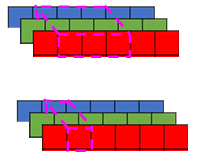
\includegraphics[width=0.9\linewidth]{figuresML_adv/lesson_ml_adv_4_pag_2.png}
    \end{minipage}
\end{figure}
\vspace{-7.5mm}

A typical example in experimental physics would be a set of particles in a detector, each carrying information about its 4-momentum vector, tracking hits, calorimeter deposits, and particle identification. We might want to pre-process them one by one identically before feeding them into a higher-level task, but this reasoning quickly hits a wall when dealing with data that do not have a fixed dimension.

\subsection{Recurrent Neural Networks (RNNs)}

To fully exploit time invariance and handle the implied causality of sequences, we must introduce a new architecture: \textbf{Recurrent Neural Networks (RNNs)}. 
But what do we actually mean by \textbf{time invariance} in a sequence? It means that the fundamental properties and the underlying meaning of a pattern do not change based on \textit{when} it occurs. Just like spatial invariance allows a CNN to recognize a specific feature regardless of its position in an image, time invariance ensures that a specific sequence of data carries the exact same meaning whether it appears at the beginning of the measurement (e.g., at $t=1$) or at the end (e.g., at $t=100$). This is exactly why an RNN can share the same weights across all time steps: the function must depend on the pattern's dynamics, not on the clock.

Unlike traditional feed-forward networks, where the information flows strictly in one direction from input to output, RNNs are iterative networks that contain a loop that allows the output of a specific step to be passed again as an input for the subsequent step. This simple but brilliant mechanism allows the network to maintain a "memory" of the previous inputs and build an internal \textbf{state} that represents what the algorithm has "understood" so far in the sequence. \\
Practically, we evaluate the network multiple times. At each time step $t$, the network takes two distinct inputs:
\begin{itemize}
    \item[-] The current element in the sequence, $X_t$.
    \item[-] The output from the previous evaluation, $h_{t-1}$ (the hidden state).
\end{itemize}

To visualize how this actually works, it is extremely useful to look at the RNN not as a single looped unit, but as an \textbf{unrolled} network over the sequence length. If we evaluate an RNN on a sequence of length $N$, we can "unroll" it into $N$ identical connected blocks, as shown in the following figure.

\begin{center}
    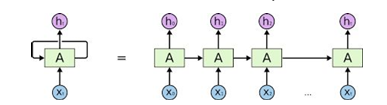
\includegraphics[width=0.5\textwidth]{figuresML_adv/lesson_ml_adv_4_pag_5.png} 
\end{center}

Pay attention to a fundamental detail: in the unrolled representation, \textit{all networks "A" are sharing the exact same weights!} We are not creating a massive, deep feed-forward network with independent layers, rather we are applying the exact same function (with the exact same parameters) at each step of the sequence. This is what guarantees the time invariance we discussed earlier: the rule to process the data does not change whether we are reading the first word of a sentence or the hundredth.

\subsection{The vanishing/exploding gradient problem}

While the concept of an RNN is elegant, training it is notoriously difficult. When we train a neural network, we use backpropagation to update the weights based on the gradient of the loss function. For an RNN, we must use a variant called \textbf{Backpropagation Through Time} (BPTT), which essentially means applying the chain rule backward through the entire unrolled network.

This leads to a critical bottleneck known as the \textbf{vanishing or exploding gradient problem}. Since the same weights are used at every step, computing the gradient for the earliest elements in a sequence requires repeatedly multiplying those weights. If the sequence is long, this repeated multiplication causes the gradient to either shrink to zero (vanishing) or grow out of control (exploding), unless the weights are perfectly around the order of 1.

{ \small
\underline{Proof:} \\
Let $\mathcal{E}$ be the total error of the network, and $\theta$ the shared weights. The total gradient is the sum of the gradients evaluated at each individual time step $t$:
\begin{equation}
    \frac{\partial \mathcal{E}}{\partial \theta} = \sum_{1 \le t \le T} \frac{\partial \mathcal{E}_t}{\partial \theta}
\end{equation}
To calculate how the error at time $t$ is affected by the state at a much earlier time $k$ (where $k < t$), we must apply the chain rule across all the intermediate steps. This introduces a product of partial derivatives:
\begin{equation}
    \frac{\partial x_t}{\partial x_k} = \prod_{i=k+1}^t \frac{\partial x_i}{\partial x_{i-1}} 
\end{equation}
Because the state $x_i$ is computed using the recurrent weights $W_{rec}$ and an activation function $\sigma$ (e.g., $x_i = \sigma(W_{rec} x_{i-1} + \dots)$), each term in the product contains $W_{rec}$. Therefore, the chain expansion becomes:
\begin{equation}
    \prod_{i=k+1}^t \frac{\partial x_i}{\partial x_{i-1}} = \prod_{i=k+1}^t W_{rec} \text{diag}(\sigma'(x_{i-1}))
\end{equation}
We are multiplying the same matrix $W_{rec}$ by itself $(t-k)$ times. If the singular values of $W_{rec}$ are strictly less than 1, this product will exponentially decay to 0, resulting in a \textbf{vanishing gradient}. Consequently, the network completely fails to learn long-term dependencies because the earlier inputs receive no gradient updates. Conversely, if the values are strictly greater than 1, the product grows exponentially, leading to an \textbf{exploding gradient} and numerical instability.
}

As a direct result of this mathematical flaw, standard RNNs are highly inefficient to train on long sequences, as they completely lose track of information that appeared too far in the past. To solve this, we must redesign the internal mechanics of the recurrent cell.

\subsection{Controlled flow of information: the birth of LSTMs}

To understand how to fix the structural flaws of standard RNNs, we can first look at how information flows through them compared to CNNs. Take a look at the following figure. As we know, CNNs are strictly focused on local correlations; far regions in an image become correlated only after several pooling layers or in the very last "flatten" step. In contrast, in a standard RNN, at every single step you are forced to process information from the \textit{entire} past. Sometimes, this is simply too much information: a network needs the ability to actively \textit{forget obsolete data} to properly work.

\begin{center}
    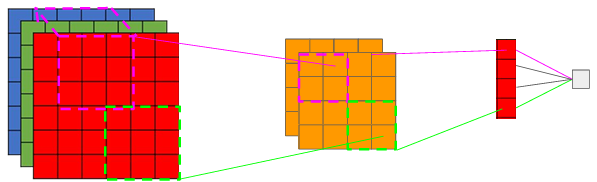
\includegraphics[width=0.55\textwidth]{figuresML_adv/lesson_ml_adv_4_pag_6.png}
    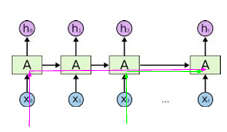
\includegraphics[width=0.32\textwidth]{figuresML_adv/lesson_ml_adv_4_pag_6a.png}
\end{center}

We are therefore facing two distinct but related problems:
\begin{enumerate}
    \item The vanishing/exploding gradient, caused by the continuous multiplication of weights across the sequence.
    \item The inability to drop useless past information.
\end{enumerate}

To solve the gradient problem, we must avoid multiplications during backpropagation. The most logical solution is to create a new, separate memory pathway called the \textbf{cell state} ($C_t$), completely distinct from the standard output hidden state ($h_t$). In this architecture the network modifies the cell state primarily via \textit{sums} rather than matrix multiplications, and since the derivative of a sum is simply 1, gradients can flow backward through time without vanishing. \\
However, this solution immediately creates a new issue. If we only \textit{add} information to the cell state at each step, the far past remains exactly as important as the recent past. We have solved the gradient problem, but we have completely destroyed any focus on locality!

To regain control over what is kept and what is discarded, we introduce \textbf{gates}. These are point-wise multiplication operations that use a sigmoid activation function to output a value strictly between 0 and 1. They act as trainable valves: if a gate outputs 0, the information is completely blocked (resetting the state); if it outputs 1, the information is left unchanged. These gates can be applied directly to the cell state (to forget past info) or to the input/output of the network.

The \textbf{Long Short-Term Memory (LSTM)} network is the very first architecture that successfully introduced and combined all these ideas.

\begin{center}
    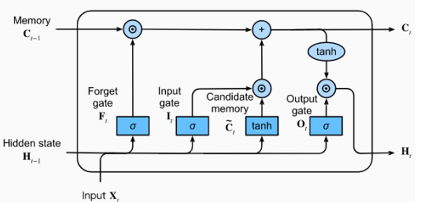
\includegraphics[width=0.75\textwidth]{figuresML_adv/lesson_ml_adv_4_pag_8.png}
\end{center}

Looking at the anatomy of an LSTM cell in the figure above, we can easily identify the mathematical implementation of our logical steps:
\begin{itemize}
    \item[-] \textbf{Forget gate ($F_t$)}: A sigmoid layer that looks at $H_{t-1}$ and $X_t$, outputting a number between 0 and 1 for each number in the cell state $C_{t-1}$. This is the network deciding what to forget.
    \item[-] \textbf{Input gate ($I_t$)} and \textbf{Candidate memory ($\tilde{C}_t$)}: Another sigmoid gate ($I_t$) decides which values we will update. Simultaneously, a $\tanh$ layer creates a vector of new candidate values ($\tilde{C}_t$) that could be added to the state.
    \item[-] \textbf{Cell State Update}: The old state $C_{t-1}$ is multiplied by $F_t$ (forgetting what we decided to drop), and then we \textit{add} $I_t * \tilde{C}_t$ (the new candidate information). This is the linear, additive path that saves our gradients!
    \item[-] \textbf{Output gate ($O_t$)}: A final sigmoid gate decides what parts of the cell state will be outputted as the new hidden state $H_t$.
\end{itemize}

Notice the rigorous choice of activation functions: sigmoids ($\sigma$) are exclusively used for the gates because we need a $0/1$ behavior, while $\tanh$ is used for the actual information to keep the internal values stabilized and bounded within a limited range.

The ultimate advantage of these gated units is their contextual adaptability. For example, when processing a text sequence, the network might learn that encountering a "space" character means the current word is over. The forget gate can use this specific trigger to reset the state, throwing away the character-level memory of the previous word and starting fresh to accumulate information for the next one.

\hrulefill

\textbf{Note: Gated Recurrent Units (GRU)}

A popular and computationally lighter alternative to the LSTM is the \textbf{Gated Recurrent Unit (GRU)}.  As you can see in the diagram below, the GRU simplifies the architecture by merging the cell state and the hidden state into a single pathway. Consequently, this also merges the input and forget gates into a single update mechanism. 

\begin{center}
    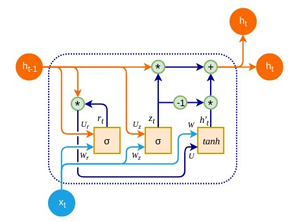
\includegraphics[width=0.4\textwidth]{figuresML_adv/lesson_ml_adv_4_pag_9.png}
\end{center}

Because of this architectural simplification, the output information is only summed, meaning there is no longer a separate, privileged path exclusively dedicated to preserving previous time step information. However, it is important to note that since all states and gates are vectors, the network still retains the ability to optimize when to forget on different timescales for different elements of those vectors.

\hrulefill

\subsection{Processing time series and architectural configurations}

One of the greatest strengths of Recurrent Neural Networks and LSTMs is their extreme architectural flexibility. Unlike standard CNNs or MLPs that require a fixed input and output size, recurrent networks can be easily adapted to process variable numbers of inputs and outputs. 

Depending on the specific task, we can arrange the unrolled network into different configurations (some represented below):
\begin{itemize}
    \item[-] \textbf{One-to-One}: This is essentially the standard feed-forward behavior, processing a single input to produce a single output.
    \item[-] \textbf{One-to-Many}: A single input is used to generate a sequence of outputs (e.g. image captioning, where one image generates a sentence of words).
    \item[-] \textbf{Many-to-One}: A sequence of inputs is processed to produce a single output. In this configuration, we typically ignore the intermediate outputs and \textit{just take the final cell state} to make our prediction (e.g. sentiment analysis of a text).
    \item[-] \textbf{Many-to-Many (Synchronous)}: We get exactly one output for each input step. The network produces a sequence of the exact same length as the input sequence (e.g. classifying every single frame of a video in real-time).
    \item[-] \textbf{Many-to-Many (Asynchronous)}: The input sequence and the output sequence have different, variable lengths. This is arguably the most useful architecture for complex tasks like text translation, and it requires a specific setup known as the Encoder-Decoder architecture.
\end{itemize} 

\begin{center}
    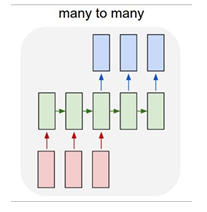
\includegraphics[width=0.3\textwidth]{figuresML_adv/lesson_ml_adv_4_pag_11.png}
    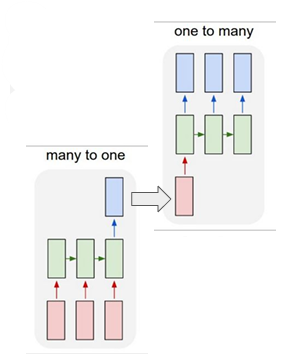
\includegraphics[width=0.35\textwidth]{figuresML_adv/lesson_ml_adv_4_pag_11a.png}
\end{center}

When we need to map an input sequence to an output sequence of a different length, we cannot rely on a simple synchronous mapping. Instead, we use our well known \textit{encoder-decoder} (or \textit{Sequence2Sequence}) architecture, which is realized by combining two separate RNNs as shown in the figure below.

\begin{center}
    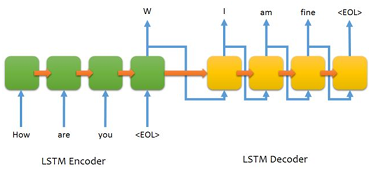
\includegraphics[width=0.5\textwidth]{figuresML_adv/lesson_ml_adv_4_pag_11b.png}
\end{center}

We have seen before how the logic behind this can be beautifully simple yet extremely powerful:
\begin{enumerate}
    \item \textit{The encoder}: The first RNN processes the input sequence step by step. Its sole purpose is to compress all the variable-length information of the sequence into a fixed-dimension latent space. Once the input sequence is over, the final \textit{cell state} of this encoder contains the "meaning" of the entire sequence.
    \item \textit{The decoder}: The second RNN takes over to generate the new sequence. Crucially, the final cell state of the encoder is explicitly passed as the \textit{initial state} for the decoder. The decoder then decompresses this state step by step to build the output.
\end{enumerate}

Since the output sequence has a variable length, the decoder needs to know when to stop generating new elements. To solve this, we must define a specific \textit{STOP token} (such as \texttt{<EOL>}, End-Of-Line). The decoder will continue to generate outputs iteratively until it predicts this exact token, at which point the generation halts.

\subsection{Data formatting and sequence management}

Before feeding data into an LSTM, the input sequence is often pre-processed element by element. In modern Deep Learning, this is typically done through an embedding layer, which maps discrete variables (like words or categorical features) into dense, continuous vectors of a fixed dimension.

Consequently, the data tensor passed to the recurrent layers usually possesses three dimensions:
\begin{itemize}
    \item[-] $N$: The batch size, i.e. number of independent sequences processed simultaneously.
    \item[-] $L$: The sequence length: while sequences can theoretically have variable lengths, in practice, to perform parallel tensor calculus on a GPU, we must define a fixed maximum length.
    \item[-] $F$: The number of features per element, or the dimension of the embedding space.
\end{itemize}

Since we force sequences into a fixed maximum length $L$, shorter sequences must be \textbf{padded} (usually with zeros) to fit the tensor. However, padding introduces a subtle but dangerous problem: if the network processes a long string of zeros at the end of a sequence, it might "learn from padding" or dilute the valuable information stored in its cell state before reaching the final output.

To prevent this, several theoretical and practical countermeasures can be implemented:
\begin{itemize}
    \item[-] \textit{Masking layers}: These explicitly tell the network to ignore padded values, skipping the computation for those specific steps.
    \item[-] \textit{Reversing the sequence order}: By feeding the sequence backward, the padding occurs at the beginning. This ensures that the actual meaningful data is processed last, meaning the "freshest" memory in the final cell state corresponds to the most important information.
    \item[-] \textbf{Bidirectional RNNs}: Instead of processing the sequence only left-to-right, a Bidirectional RNN processes it simultaneously in both directions using two separate hidden states. This ensures that the network has both past and future context at every single step of the sequence, making it incredibly robust.
\end{itemize}

\subsection{Practical implementation in PyTorch and Keras}

Now that we have established the theoretical foundations of sequence processing, let's take a look at how we can actually code these architectures. First, some general notions on how PyTorch and Keras handle LSTM layers and sequence management that can be useful for your software.

When defining an LSTM in PyTorch, you must pay close attention to the expected input shape. By default, PyTorch uses a "batch second convention", meaning it expects tensors formatted as \texttt{(Sequence, Batch, Features)}. While this is implemented as a memory optimization under the hood, it is generally counterintuitive and not strictly relevant for standard toy examples or simpler problems. Therefore, it is highly suggested to use the \texttt{batch\_first=True} option, which restores the more standard \texttt{(Batch, Sequence, Features)} shape for an easier understanding of the code.

Here is a typical initialization:

\begin{verbatim}
import torch.nn as nn

lstm = nn.LSTM(input_size=10, hidden_size=20, batch_first=True)
output, (h_n, c_n) = lstm(input_batch)
\end{verbatim}

As you can see, evaluating the LSTM layer explicitly returns three distinct objects:
\begin{enumerate}
    \item \texttt{output}: The hidden features for each time step in the sequence. Its shape will be \texttt{(Batch, Seq, Hidden)}.
    \item \texttt{h\_n}: The hidden state of the very last step. Its shape will be \texttt{(Num Layers, Batch, Hidden)}.
    \item \texttt{c\_n}: The cell state of the very last step.
\end{enumerate}

Furthermore, to avoid performing pointless calculations on padded zero-values (as we discussed in the previous section), PyTorch implements an elegant optimization using the \texttt{PackedSequence} class. This method removes the zeros while keeping track of the original indices, computes the math through the LSTM, and finally places the zeros back in their correct positions:

\begin{verbatim}
packed_input = pack_padded_sequence(input, lengths)
# LSTM evaluation returning packed_output
output = pad_packed_sequence(packed_output)
\end{verbatim}

The logic is incredibly similar in Keras. An LSTM layer can be configured to return just the output of the last iteration, the whole sequence of outputs, the gated output of the memory (the hidden state), and the cell state. 

We can control this behavior using the \texttt{return\_sequences} and \texttt{return\_state} boolean parameters:

\begin{verbatim}
from keras.models import Model
from keras.layers import Input, LSTM
from numpy import array

inputs1 = Input(shape=(5, 1))
lstm1, state_h, state_c = LSTM(1, return_state=True, return_sequences=True)(inputs1)
model = Model(inputs=inputs1, outputs=[lstm1, state_h, state_c])

data = array([0.1, 0.2, 0.3, 0.4, 0.5]).reshape((1, 5, 1))
print(model.predict(data))

[Output]
1/1 [==============================] - 0s 145ms/step
[array([[[0.01334215],
         [0.03582103],
         [0.06321989],
         [0.09452317],
         [0.12837262]]], dtype=float32), 
 array([[0.12837262]], dtype=float32), 
 array([[0.2541938 ]], dtype=float32)]
\end{verbatim}

If you run this code, the output will contain three distinct arrays: the full sequence of 5 hidden states, the final hidden state (\texttt{state\_h}), and the final cell state (\texttt{state\_c}). You will immediately notice that the specific value of \texttt{state\_h} perfectly matches the exact last element of the \texttt{lstm1} sequence array, mathematically confirming that the network is outputting the final time-step representation alongside the full sequence history.

\section{Hands-on examples for LSTMs}

To put these concepts into practice, the accompanying exercises involve building LSTM architectures for two different sequence tasks.

\begin{itemize}
    \item[-] \textit{LSTM Encoder Exercise}: We try building from scratch an LSTM that, given a sequence of two-dimensional vectors, finds the maximum norm and the position in the sequence. We will need to generate some data and build a network with one LSTM layer followed by a Dense one. Here is the link to the Notebook: \url{https://colab.research.google.com/drive/1m9Ybt08aNbNNJgVCVEWa03bnfaNqaNJh?usp=sharing}.
    \item[-] \textit{LSTM Decoder exercise}: We will teach multiplication tables to our LSTM. We give the network a base $B$ and a number $N$ of values we want, and it should produce a sequence $[1*B, 2*B, \dots, N*B]$. Let's try to use an "end of sequence" token (e.g., -1). Here is the link to the Notebook: \url{https://colab.research.google.com/drive/10waGCBQG_iDC2ewYZKGjUBR3YQ50BnO7?usp=sharing}
\end{itemize}

Since I have to start a new page in order to input the Notebook in my LaTeX file, here is a compilation of photos from the Grand Slam Tournaments of 1989. In order:
\begin{itemize}
    \item[-] Ivan Lendl with the 1989 Australian Open trophy (\textit{upper left});
    \item[-] Michael Chang after winning the 1989 Roland Garros against Stefan Edberg (after eliminating Ivan Lendl in the quarterfinals in a legendary match of psychological warfare, \textit{upper right});
    \item[-] Boris Becker after winning the 1989 Wimbledon final against Stefan Edberg (\textit{bottom left});
    \item[-] Steffi Graf and Boris Becker after winning the 1989 Men's and Women's singles at the US Open for Germany (\textit{bottom right}).
\end{itemize}

\begin{center}
    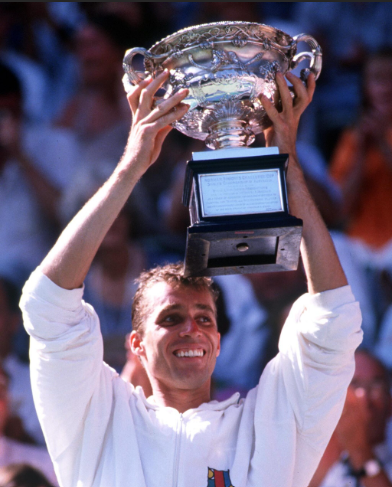
\includegraphics[width=0.23\textwidth]{figuresML_adv/ivan_lendl_1989.png}
    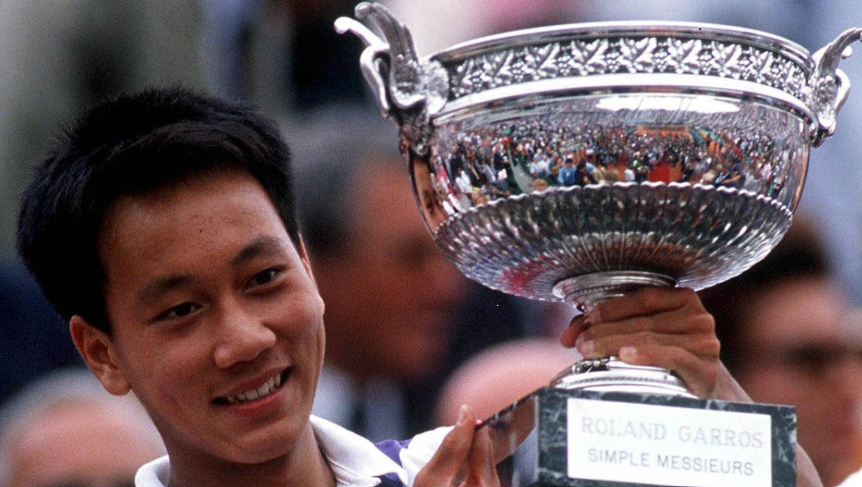
\includegraphics[width=0.5\textwidth]{figuresML_adv/michael_chang_1989.png}
\end{center}
\begin{center}
    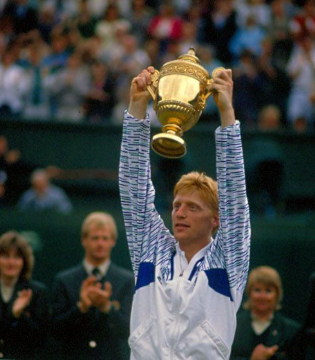
\includegraphics[width=0.25\textwidth]{figuresML_adv/boris_becker_1989.png}
    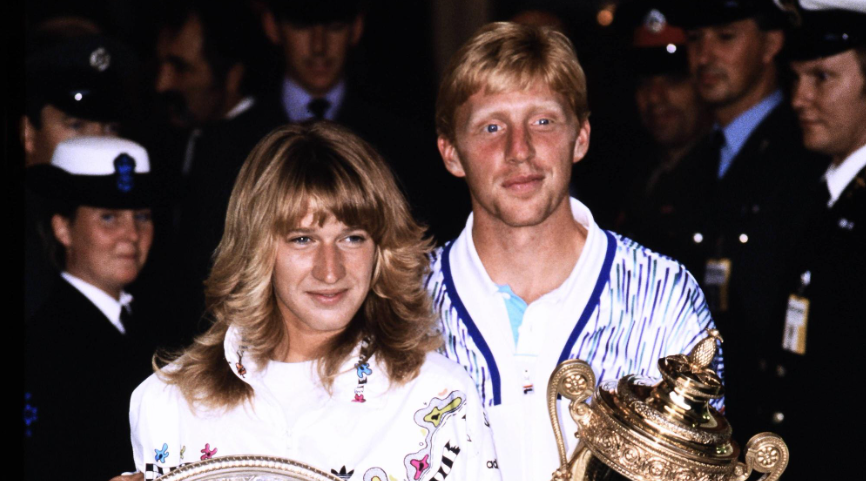
\includegraphics[width=0.5\textwidth]{figuresML_adv/becker_graff_1989.png}
\end{center}


%\includepdf[pages=-, pagecommand={\thispagestyle{plain}}]{lezioni/e_ML_adv_4ahands_on.pdf}
%ML_8a nel mio colab

%\includepdf[pages=-, pagecommand={\thispagestyle{plain}}]{lezioni/e_ML_adv_4bhands_on.pdf}
%ML_8b nel mio colab